\documentclass{resume}

\begin{document}

\fontfamily{ppl}\selectfont

\noindent
\begin{tabularx}{\linewidth}{@{}m{0.8\textwidth} m{0.2\textwidth}@{}}
{
    \Large{Bernardo Paulsen} \newline
    \small{
        \clink{
            \href{mailto:bernardopaulsen@gmail.com}{bernardopaulsen@gmail.com} \textbf{·} 
            {\fontdimen2\font=0.75ex +55 (51) 981 441 383} 
            \textbf{·} 
            \href{https://bernardopaulsen.github.io}{bernardopaulsen.github.io}
        } \newline
        Porto Alegre, Brasil
    }
} & 
{
    \hfill
    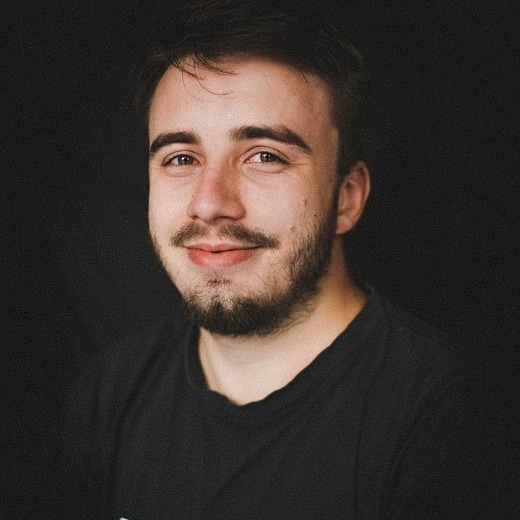
\includegraphics[width=2.8cm]{images/gr.jpg}
}
\end{tabularx}
\begin{center}
\begin{tabularx}{\linewidth}{@{}*{2}{X}@{}}
% left side %
{
    \csection{Experiência}{\small
        \begin{itemize}
            \item \frcontent{Argentum Investimentos}{Asssessor de Investimentos}{Prospecção, atendimento de clientes e backoffice.}{Abril de 2019 a outubro de 2019}
            \item \frcontent{Argentum Investimentos}{Estagiário}{Prospecção de clientes e backoffice.}{Setembro de 2018 a março de 2019}
            \item \frcontent{Equilíbrio Assessoria Econômica}{Gerente de Projeto}{Gerência do projeto \href{https://github.com/bernardopaulsen/Relatorio-de-Conjuntura}{Relatório de Conjuntura}}{Janeiro de 2017 a dezembro de 2017}
            \item \frcontent{Equilíbrio Assessoria Econômica}{Assessor}{Assessor da Diretoria de Projetos.}{Julho de 2016 a dezembro de 2016}
        \end{itemize}
    }
    \csection{Educação}{\small
        \begin{itemize}
            \item \frcontent{Mestrado Profissional em Economia}{Universidade Federal do Rio Grande do Sul}{}{Previsão: 2021}
            \item \frcontent{Graduação em Ciências Econômicas}{Universidade Federal do Rio Grande do sul}{}{2019}
        \end{itemize}
    }
    \csection{Cursos}{\small
        \begin{itemize}
            \item \frcontent{Learn Complete Python}{DURGASOFT DURGA, Software Training Organization}{}{Previsão: 2021}
        \end{itemize}
    }
} 
% end left side %
& 
% right side %
{
    \csection{Habilidades}{\small
        \begin{itemize}
            \item \textbf{Linguagens de Programação/Discrição} \newline
            {\footnotesize }{Python, \LaTeX, Git, R}{}
            \item \textbf{Programas} \newline
            {\footnotesize }{Gretl, Excel}{}
            \item \textbf{Idiomas} \newline
            {\footnotesize }{Inglês, Espanhol}{}
        \end{itemize}
    }
    \csection{Projetos no \href{https://github.com/bernardopaulsen}{Github}}{\small
        \begin{itemize}
            \item \frcontent{Thesis}{Dissertação de mestrado.}{}{Python}
            \item \frcontent{Import}{Bibliotecas para importação de dados do Yahoo! Finance e BACEN SGS via API.}{}{Python}
            \item \frcontent{Website}{Website pessoal.}{}{\LaTeX}
            \item \frcontent{Games}{Jogos simples.}{}{Python}
        \end{itemize}
    }
    \csection{Hobbies \& Interesses}{\small
        \vspace{0.32cm}
        \begin{tabularx}{\linewidth}{@{}*{4}{>{\centering\arraybackslash}X}@{}}
            {\centering
            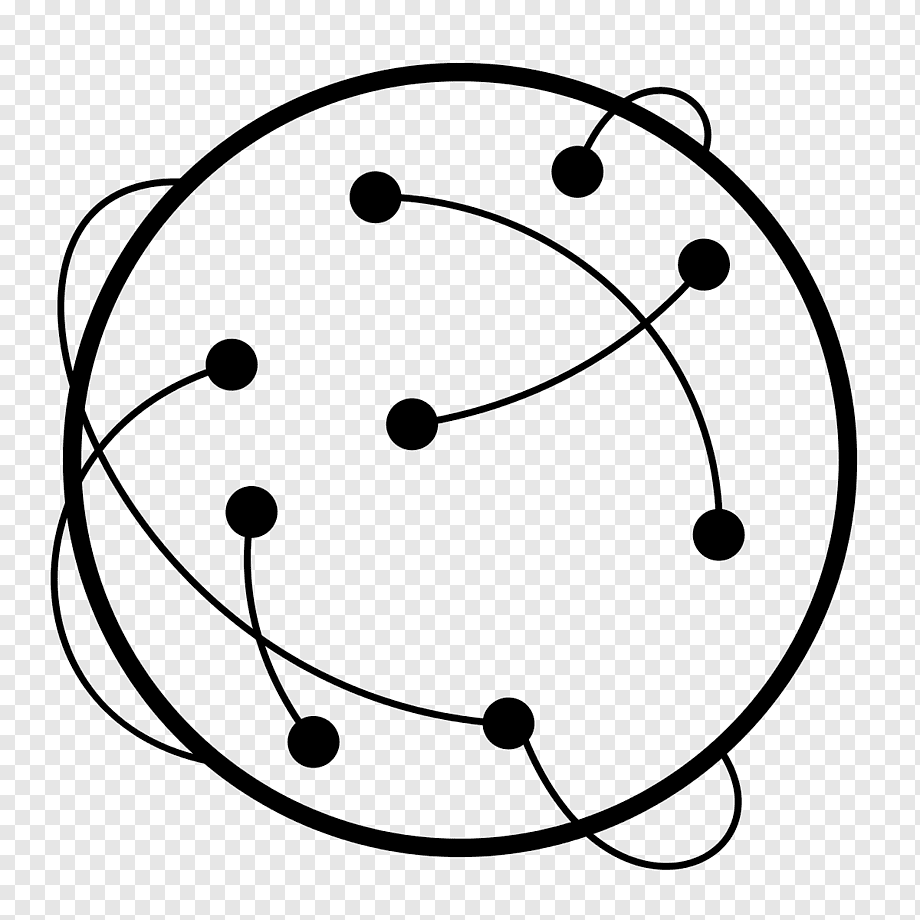
\includegraphics[width=0.8cm]{images/science.png}
            } &
            {\centering
            
\includegraphics[width=0.8cm]{images/pricing.png}
            } & 
            {\centering
            
\includegraphics[width=0.8cm]{images/reading.png}
            } &
            {\centering
            
\includegraphics[width=0.8cm]{images/sports.jpg}
            } \\
            {\footnotesize Ciência de Dados} & {\footnotesize Precificação de Ativos} & {\footnotesize Leitura} & {\footnotesize Esportes}
        \end{tabularx}
    }
}
\end{tabularx}
\end{center}
\end{document}